\documentclass[aspectratio=169, 12pt]{beamer}
% \documentclass[aspectratio=169, handout]{beamer} % for handout
\usepackage{pgfpages}
\usepackage[english]{babel}
\usepackage{booktabs,listings}
\usepackage[T1]{fontenc}
\usepackage[utf8]{inputenc}
\usepackage{xcolor}
\usepackage{graphicx}
\usepackage{graphics}
\usepackage{epstopdf}
\usepackage{upgreek}
\usepackage{amsmath}
\usepackage{textcomp}
\usepackage{booktabs}
\usepackage{tikz}
\usetikzlibrary{positioning,shapes,arrows,calc}
\usepackage{adjustbox}
\usepackage{siunitx}
\newcommand{\mesunt}[1]{\left[\si{#1}\right]}

\lstset{basicstyle=\ttfamily}
\setlength{\parskip}{.5\baselineskip}
\usetheme[style=vertical, frametotal=true]{NTNU}

\mode<handout>{%
    \pgfpagesuselayout{2 on 1}[a4paper] 
    % \setbeameroption{show notes}
}


\title{ Repartition of inertia service between wind turbine and battery in power systems }
% \subtitle{Project for the ET8301 course}
\author{Andreetta Niccolò}
\date{May $31^{st}$ 2024}

\begin{document}
  \maketitle

  \begin{frame}[fragile]{Outline}
    \tableofcontents
  \end{frame}

  \section{Background and problem statement}
  \begin{frame}{\insertsection}
    Increase of energy from renewable energy resources implies lost of inertia in the grid. 

    One possible solution is gain inertia controlling the converters to act as synchronous machines (debate about that approach).

    \begin{figure}
      \centering
      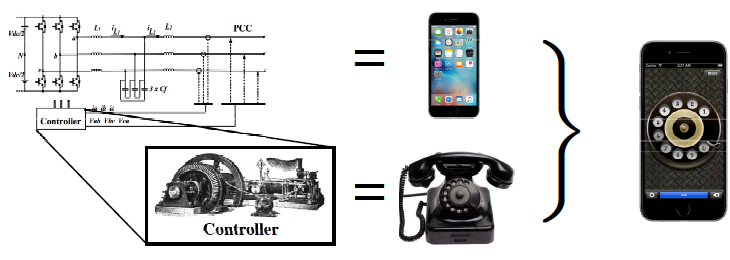
\includegraphics[width = 0.5\columnwidth]{florian_phone.png}
    \end{figure}
  \end{frame}
  
  \section{Research questions}
  \begin{frame}{Research questions}
    \textcolor{NTNUBlue}{Main question}: Which is the most effective way to provide inertia when a wind turbine and a battery are available in a power system?
    
    \textcolor{NTNUOrange}{Solution idea}: Allocate the amount of power between the available in the most economic way
  \end{frame}
  
\end{document}